\documentclass[a4paper]{article}
\usepackage{cmap}
\usepackage[utf8]{inputenc}
\usepackage[T2A]{fontenc}
\usepackage[english,russian]{babel} 
\usepackage[left=15mm, top=15mm, right=15mm, bottom=42mm, nohead, nofoot]{geometry}
\usepackage{blindtext}  % рыба-текст
\usepackage{graphicx}  % изобржаения
\usepackage{float} % плавающие объекты
\usepackage{wrapfig}  % изобржаения
\usepackage{tikz} % графика
\usepackage{mdframed} % рамки
\usepackage{xcolor} % определение цветов
\usepackage{nicefrac} % красивые дроби
\usepackage{cancel} % сокращение
\usepackage{amsmath,amsfonts,amssymb} % математический пакет
\usepackage{hyperref}  % гиперссылки
\usepackage{fancybox,fancyhdr} % хедер и футер
\usepackage{listings} % код
\pagestyle{fancy}
\fancyhf{}
\fancyhead[L]{Теория вероятности}
\fancyhead[C]{Рубежный тест №1}
\fancyhead[R]{25.04.2024}
\fancyfoot[C]{\thepage}
\headsep=8mm
\footskip=20mm

\definecolor{urlcolor}{HTML}{3454D1}
\definecolor{linkcolor}{HTML}{3454D1}
\hypersetup{pdfstartview=FitH, linkcolor=linkcolor, urlcolor=urlcolor, colorlinks=true}

\definecolor{strings}{rgb}{0,0.6,0}
\definecolor{comments}{rgb}{0,0.3,0}
\definecolor{numbers}{rgb}{0.5,0.5,0.5}
\definecolor{keywords}{rgb}{0.09,0.61,0.95}
\definecolor{background}{rgb}{0.97,0.97,0.97}
\lstdefinestyle{codestyle}{
    backgroundcolor=\color{background},
    commentstyle=\color{comments},
    keywordstyle=\color{keywords},
    stringstyle=\color{strings},
    numberstyle=\tiny\color{numbers},
    basicstyle=\ttfamily\footnotesize,
    breakatwhitespace=false,
    breaklines=true,
    captionpos=b,
    inputencoding=utf8,
    keepspaces=true,
    numbers=left,
    numbersep=5pt,
    showspaces=false,
    showstringspaces=false,
    showtabs=false,
    tabsize=2,
    extendedchars=true,
    literate=
    {а}{{\cyra}}1
    {б}{{\cyrb}}1
    {в}{{\cyrv}}1
    {г}{{\cyrg}}1
    {д}{{\cyrd}}1
    {е}{{\cyre}}1
    {ж}{{\cyrzh}}1
    {з}{{\cyrz}}1
    {и}{{\cyri}}1
    {й}{{\cyrishrt}}1
    {к}{{\cyrk}}1
    {л}{{\cyrl}}1
    {м}{{\cyrm}}1
    {н}{{\cyrn}}1
    {о}{{\cyro}}1
    {п}{{\cyrp}}1
    {р}{{\cyrr}}1
    {с}{{\cyrs}}1
    {т}{{\cyrt}}1
    {у}{{\cyru}}1
    {ф}{{\cyrf}}1
    {х}{{\cyrh}}1
    {ц}{{\cyrc}}1
    {ч}{{\cyrch}}1
    {ш}{{\cyrsh}}1
    {щ}{{\cyrshch}}1
    {ъ}{{\cyrhrdsn}}1
    {ы}{{\cyrery}}1
    {ь}{{\cyrsftsn}}1
    {э}{{\cyrerev}}1
    {ю}{{\cyryu}}1
    {я}{{\cyrya}}1
    {А}{{\CYRA}}1
    {Б}{{\CYRB}}1
    {В}{{\CYRV}}1
    {Г}{{\CYRG}}1
    {Д}{{\CYR96}}1
    {Е}{{\CYRE}}1
    {Ж}{{\CYRZH}}1
    {З}{{\CYRZ}}1
    {И}{{\CYRI}}1
    {Й}{{\CYRISHRT}}1
    {К}{{\CYRK}}1
    {Л}{{\CYRL}}1
    {М}{{\CYRM}}1
    {Н}{{\CYRN}}1
    {О}{{\CYRO}}1
    {П}{{\CYRP}}1
    {Р}{{\CYRR}}1
    {С}{{\CYRS}}1
    {Т}{{\CYRT}}1
    {У}{{\CYRU}}1
    {Ф}{{\CYRF}}1
    {Х}{{\CYRH}}1
    {Ц}{{\CYRC}}1
    {Ч}{{\CYRCH}}1
    {Ш}{{\CYRSH}}1
    {Щ}{{\CYRSHCH}}1
    {Ъ}{{\CYRHRDSN}}1
    {Ы}{{\CYRERY}}1
    {Ь}{{\CYRSFTSN}}1
    {Э}{{\CYREREV}}1
    {Ю}{{\CYRYU}}1
    {Я}{{\CYRYA}}1
}

\lstset{style=codestyle}

\addto\captionsrussian{
  \renewcommand{\contentsname}
    {\centering Содержание}
}
\newcommand{\addsection}[1]{
    \phantomsection
    \addcontentsline{toc}{section}{#1}
    \section*{\centering #1}
}
\newcommand{\addsubsection}[1]{
    \phantomsection
    \addcontentsline{toc}{subsection}{#1}
    \subsection*{\centering #1}
}
\newcommand{\addsubsubsection}[1]{
    \phantomsection
    \addcontentsline{toc}{subsubsection}{#1}
    \subsubsection*{\centering #1}
}

\newmdenv[
  leftmargin = 0.5em,
  skipabove = 0.5em,
  skipbelow = 0.5em,
  linewidth = 1pt,
  rightline = false,
  topline = false,
  bottomline = false
]{quotebox}

\newlength{\tempheight}
\newcommand{\Let}{
\mathbin{\text{\settoheight{\tempheight}{\mathstrut}\raisebox{0.4\pgflinewidth}{
\tikz[baseline=0.5ex,line cap=round,line join=round] \draw (0,0) --++ (0.3em,0) --++ (0,2.3ex) --++ (-0.3em,0);
}}}}
\newcommand*\squared[1]{\tikz[baseline=(char.base)]{
            \node[shape=rectangle,draw,inner sep=4pt] (char) {#1};}}
\newcommand*\msquared[1]{\tikz[baseline=(char.base)]{
            \node[shape=rectangle,draw,inner sep=4pt] (char) {$\displaystyle #1$};}}
\newcommand{\at}{\biggr\rvert}
\newcommand{\shiftright}[3]{\makebox[#2][r]{\makebox[#1][l]{#3}}}
\newcommand{\e}{\;\text{e}}
\let\oldint\int
\def\int{\oldint\limits}
\DeclareRobustCommand{\divby}{%
  \mathrel{\vbox{\baselineskip.65ex\lineskiplimit0pt\hbox{.}\hbox{.}\hbox{.}}}%
}

\newcommand\NB{\textbf{N\kern-0.32em\textcolor{red}{B}}}

\begin{document}
\noindent ФИО/Поток: \underline{Овчинников Павел Алексеевич, ТеорВер 1.2}\rule[-1.25mm]{8.6cm}{0.15mm}\\[1em]
\addsubsection{Задание №1}
(b) Да, является, т.к. выполняет все условия, необходимые для того, чтобы быть алгеброй:
\begin{itemize}
    \item $\Omega \in \mathbf{F}$,
    \item $\forall A, B \in \mathbf{F} \Rightarrow A \cup B \in \mathbf{F}\quad(A, B, A + B \in \mathbf{F})$,
    \item $\forall A \in \mathbf{F} \Rightarrow \bar{A} \in \mathbf{F}$, где $\bar{A} = \Omega \setminus A$.
\end{itemize}
\addsubsection{Задание №2}
(a) Да, является, потому как выполняются все свойства сигма-алгебры:
\begin{itemize}
    \item $\varnothing \in \mathcal{F}$
    \item $\forall A \Rightarrow \bar{A} \in \mathcal{F}\quad(\bar{A}, \bar{B}, \overline{A + B}, \overline{\bar{A} + \bar{B}} \in \mathcal{F})$
    \item $\cup^\infty_{i=1} A_i \in \mathcal{F}\quad(A + B \in \mathcal{F})$
\end{itemize}
\addsubsection{Задание №3}
(a) Да, существует. Для того, чтобы проверить существование вероятностного пространства, необходимо воспользоваться формулой включений-исключений:
$$P(A + B + C) = P(A) + P(B) + P(C) - P(AB) - P(BC) - P(AC) + P(ABC)$$
$$0.9 = 0.4 + 0.52 + 0.46 - 0.25 - 0.13 - 0.14 + 0.04$$
$$0.9 = 0.92 + 0.21 - 0.23$$
$$0.9 = 0.9$$
Принцип выполняется, поэтому вероятностное пространство существует.\\[0.5em]
(b) Нет, не существует. Нам необходимо вычислить из имеющихся условий дополнительно $P(AB), P(AC), P(BC), P(ABC)$.
$$P(AB) = P(A) + P(B) - P(A + B) = 0.3 + 0.4 - 0.6 = 0.1$$
$$P(BC + AC) = P(BC) + P(AC) - P(ABC) = 0 \Rightarrow P(ABC) = P(BC) + P(AC)$$
Подставляем в итоговую формулу включений-исключений:
$$P(A + B + C) = P(A) + P(B) + P(C) - P(AB) - \cancel{P(BC) - P(AC)} + \cancel{P(BC) + P(AC)}$$
$$0.7 = 0.3 + 0.4 + 0.2 - 0.1$$
$$0.7 = 0.7 + 0.1$$
$$0.7 \neq 0.8$$
\addsubsection{Задания №6}
Нет, отображение $X$ не является случайной величиной, поскольку каждому событию $A_i$ сопоставляется отрицательное числовое значение.
\addsubsection{Задания №7}
(a) Нет, т.к. функция распределения случайной величины $F(x)$ не может убывать и должна всегда расти ввиду её свойства по плотности вероятности $F(x) = \int\nolimits_{-\infty}^{x}\varphi(x)\,dx$.\\[0.5em]
(b) Нет, т.к. функция распределения случайной величины всегда достигает 1 с ростом $x$. Здесь же мы этого не наблюдаем в рамках графика.\\[0.5em]
(c) Да, потому как соответствует выше озвученным условиям.\\[0.5em]
(d) Нет, т.к. часть графика вышла за границы 1 --- такое недопустимо для графика функции распределения случайной величины.
\addsubsection{Задание №9}
Да, эта функция является функцией распределения случайной величины. Такая функция должна удовлетворять трём условиям: непрерывность слева, монотонно не убывающая, $\lim_{t\rightarrow -\infty} F(t) = 0$ и $\lim_{t\rightarrow \infty} F(t) = 1$. Все три функции удовлетворяют этим условиям, поэтому удовлетворяет и исходная функция. Но только потому, что в сумме все коэффициенты перед функциями распределения равны 1. Если коэффициент 0.5 заменить на 0.6, то, тогда $\lim_{t\rightarrow \infty} F(t) = 1.1$.
\addsubsection{Задание №10}
\begin{figure}[H]
    \centering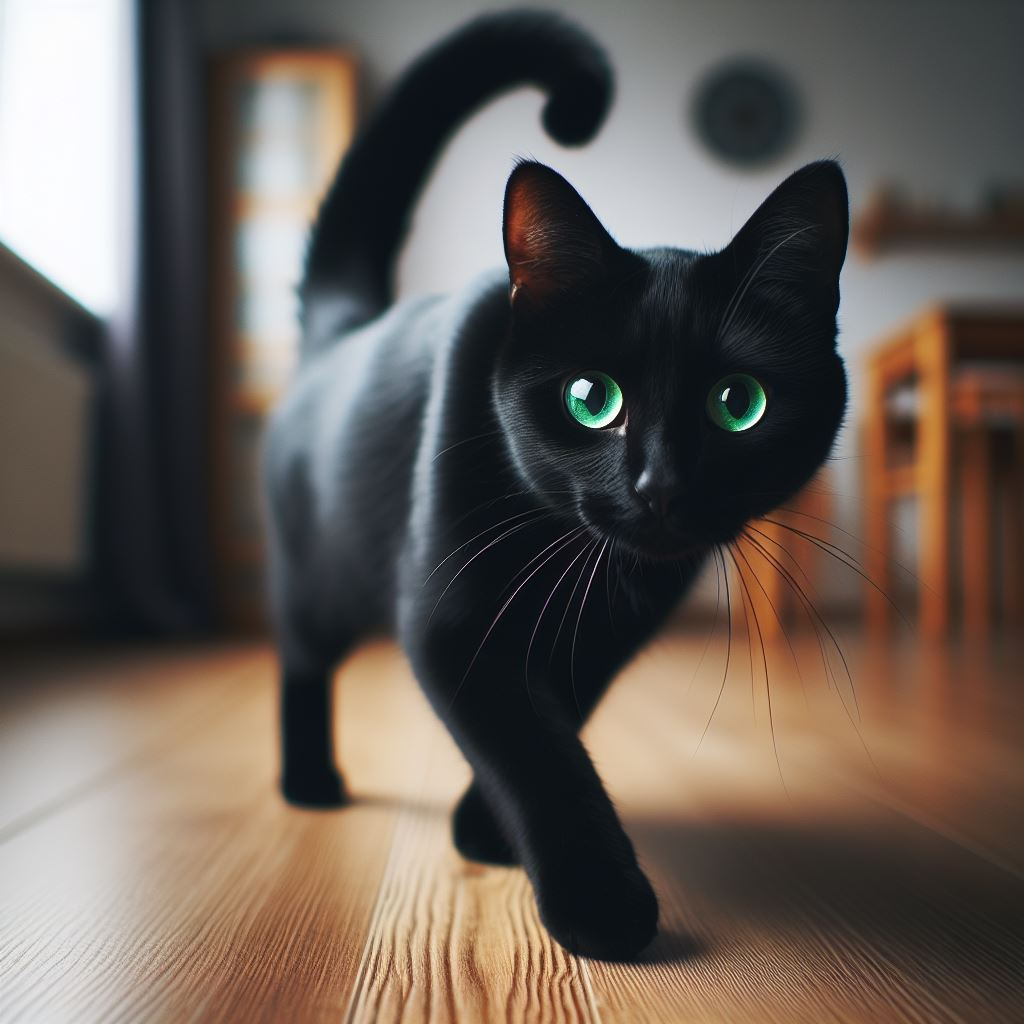
\includegraphics[width=0.5\textwidth]{kitten.jpeg}
    \caption{Картинка сгенерирована нейросетью.}
\end{figure}
\end{document}